\renewcommand{\theequation}{\theenumi}
\renewcommand{\thefigure}{\theenumi}
\renewcommand{\thetable}{\theenumi}
\begin{enumerate}[label=\thesection.\arabic*.,ref=\thesection.\theenumi]
\numberwithin{equation}{enumi}
\numberwithin{figure}{enumi}
\numberwithin{table}{enumi}


\item In the following table, $X$ is a discrete random variable and $p(X=x)$ is the probability density. The standard deviation of $X$ is 
%
\begin{table}[h!]
    \centering
    \begin{tabular}{|c|c|c|c|}
        \hline
        $X$ & 1 & 2 & 3  \\
        \hline
        $p_X(k)$ & 0.3 & 0.6 & 0.1\\
        \hline
    \end{tabular}
    \label{cond/1/tab:my_label}
    \caption{Probability Distribution}
\end{table}
\\
\solution
From the given information,
%
\begin{align}
    \mu&= \sum_{k=1}^3 k p_X(k)\\
    &=1.8
\end{align}
and 
\begin{align}
    \sigma^2 &= E(X^2) -\mu^2\\
    &= \sum_{k=1}^3 k^2 p_X(k) - \mu^2\\
    &= 0.36 \\
    \implies 
    \sigma &= 0.6
\end{align}
%
\item An urn contains 5 red balls and 5 black balls.In the first draw, one ball is picked at random and discarded without noticing its colour.The probability to get a red ball in the second draw is

\begin{enumerate}
\begin{multicols}{4}
\setlength\itemsep{2em}

\item $\dfrac{1}{2}$
\item $\dfrac{4}{9}$
\item $\dfrac{5}{9}$
\item $\dfrac{6}{9}$
\end{multicols}
\end{enumerate}
\solution
Let $X_i \in \cbrak{0,1}$ represent the $i^{th}$ draw where 1 denotes a red ball is drawn.

\begin{table}[h]
\centering 
\caption{}
\begin{tabular}{|c|c|c|}
\hline
           & $X_1 = 0$ & $X_1 = 1$\\
\hline
$X_2 = 0$  & 4/18      & 5/18  \\
\hline
$X_2 = 1$  & 5/18      & 4/18  \\
\hline
\end{tabular}
\label{table:}
\end{table}
 
Table \ref{table:} represents the probabilities of all possible cases when two balls are drawn one by one from the urn.

\begin{align}
    \pr{X_2 = 1} &= \pr{X_2 = 1|X_1 = 0}+\pr{X_2 = 1|X_1 = 1}\\
                 &=\frac{5}{18}+\frac{4}{18} \\
                 &= \frac{1}{2}
\end{align}
The required option is (A).
%
\item Out of all the 2-digit integers between 1 and 100, a 2-digit number has to be selected at random. What is the probability that the selected number is not divisible by 7?
\begin{enumerate}[label = (\Alph*)]
\item $\frac{13}{90}$\\
\item $\frac{12}{90}$\\
\item $\frac{78}{90}$\\
\item $\frac{77}{90}$
\end{enumerate}
%
\solution
Let $X = \cbrak{10,11, \ldots, 99}$ be a random variable. Here, $\floor*{x}$ rounds off $x$ to the greatest integer less than $x$.
\begin{align}
    \pr{X \tpmod{7}\neq 0} &= 1 - \frac{n(X \tpmod{7}= 0)}{n(X)}\\
    &= 1 -  \frac{\floor*{\frac{100}{7}}- \floor*{\frac{10}{7}}}{90} \\
    &= 1 - \frac{13}{90}\\
    &= \frac{77}{90}
\end{align}
So, the correct option is (D).
%



\item There are 3 red socks, 4 green socks and 3 blue socks.You choose 2 socks.The probability that they are of the same colour is

\begin{enumerate}
\begin{multicols}{4}
\setlength\itemsep{2em}

\item $\dfrac{1}{5}$
\item $\dfrac{7}{30}$
\item $\dfrac{1}{4}$
\item $\dfrac{4}{15}$

\end{multicols}
\end{enumerate}
\solution
Let $X_i \in \cbrak{1, 2, 3}$ represent the $i^{th}$ draw, where 1, 2, 3 correspond to the colour of socks drawn as Red, Blue and Green respectively
\begin{table}[ht]
\centering 
\caption{}
\begin{tabular}{|c|c|c|c|}
\hline
           & $X_1 = 1$ & $X_1 = 2$ & $X_1 = 3$\\
\hline
$X_2 = 1$  & 6/90      & 12/90     & 9/90  \\
\hline
$X_2 = 2$  & 12/90      & 12/90    & 12/90  \\
\hline
$X_2 = 3$  & 9/90      & 12/90    & 6/90  \\
\hline
\end{tabular}
\label{table}
\end{table}
  
TABLE  \ref{table} represents all the possibilities of choosing socks one by one.
  
 
The probability that the two socks drawn are of the same colour(by substituting values from table \ref{table})
 \begin{align}
     &= \Pr\brak{X_1 = X_2} \\
     &= \sum_{i = 1}^3 \Pr\brak{X_2 = i | X_1 = i}\Pr\brak{X_1 = i}\\
     &= \dfrac{6}{90} +\dfrac{12}{90} + \dfrac{6}{90}\\
     &= \dfrac{4}{15}
 \end{align}
 So the correct option is (D)

\item The probability that a \textit{k}-digit number does NOT contain the digits 0,5, or 9 is

\begin{enumerate}
\begin{multicols}{4}
\setlength\itemsep{2em}

\item $0.3^k$
\item $0.6^k$
\item $0.7^k$
\item $0.9^k$

\end{multicols}
\end{enumerate}
\solution
Let 
\begin{align}
X_{i}\in \{0,1,2, \ldots ,9\}
\end{align}
represent the digit at the $i^{th}$ place.

\begin{align}
\pr{X_i \notin \{0,5,9\}}=\frac{7}{10}=0.7     
\end{align}
If the k-digit number does not contain 0,5 or 9,
\begin{align}
\pr{X_{1} \notin \{0,5,9\} ,X_{2} \notin \{0,5,9\} ,\ldots, X_{k} \neq \{0,5,9\}  }
\end{align}
Since the events are independent, 
\begin{multline}\label{3:eq1}
  \pr{X_{1} \notin \{0,5,9\} ,X_{2} \notin \{0,5,9\} ,\ldots, X_{k} \neq \{0,5,9\}  }\\
  =  \pr{X_1 \notin \{0,5,9\}}\ldots\pr{X_k \notin \{0,5,9\}}
\end{multline}
\begin{align}
&=\prod_{i=1}^{k} 0.7\\
&=(0.7)^{k}
\end{align}

\begin{figure}[h!]
    \centering
    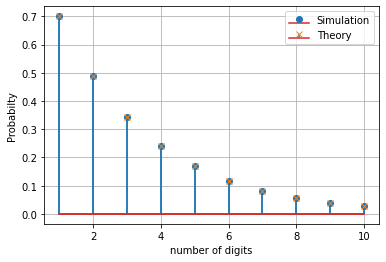
\includegraphics[width=\linewidth]{figs/3.png}
    \caption{Plot  }
    \label{3:}
\end{figure}
%
\item Candidates were asked to come to an interview with 3 pens each. Black,blue,green and red were the permitted pen colours that the candidate could bring. The probability that a candidate comes with all 3 pens having the same colour is.......
%
\item Let X and Y denote the sets containing 2 and 20 distinct objects respectively and F denote the set of all possible functions defined from X and Y. Let f be randomly chosen from F. The probability of f being one-to-one is........
%
\item Consider a dice with the property that the probability of a face with \textit{n} dots showing up is proportional to \textit{n}. The probability of the face with three dots showing up is......
%
\solution
Let X be random variable.\\
X $\in$ \{1,2,3,4,5,6\}\\
$p_{X}(n)\rightarrow$Probability of showing up n.\\
As $p_{X}(n)$ is proportional to n. We have,
\begin{align}
    p_{X}(n) = 
    \begin{cases}
        kn & 1 \leq n \leq 6 \\
        0  & otherwise
    \end{cases}
    \tag{8.1}
\end{align}
Where k is some real constant.

\begin{table}[ht]
\centering 
\caption{}
\begin{tabular}{|c|c|c|c|c|c|c|}
\hline
 n          & 1 & 2 & 3 & 4 & 5 & 6 \\
\hline
 $p_{X}(n)$ & k  & 2k & 3k & 4k & 5k & 6k\\
\hline
\end{tabular}
\label{8:table}
\end{table}

We know that,
\begin{align}
    \tag{8.2}
    \sum_{n=1}^6 p_{X}(n)=1
    \label{8:eq:1}
\end{align}
By substituting the values in \ref{8:eq:1}, we have
\begin{align}
    \tag{8.3}
    k+2k+3k+4k+5k+6k=1
\end{align}
\begin{align}
     \tag{8.4}
   \implies  k=\frac{1}{21}
   \label{8:eq:2}
\end{align}
Probability of the face with three dots showing up 
\begin{align}
    \tag{8.5}
    \implies p_{X}(3)=3k
\end{align}
Substituting the value of k from \ref{8:eq:2}
\begin{align}
    \tag{8.6}
    \implies p_{X}(3)=\frac{1}{7}
\end{align}

\item A box contains 4 white balls and 3 red balls. In succession, two balls are randomly selected and removed from the box. Given that the first removed ball is white, the probability that the second removed ball is red is
\begin{enumerate}
\begin{multicols}{4}
\setlength\itemsep{2em}
\item $
\dfrac{1}{3}
$
\item $
\dfrac{3}{7}
$
\item $
\dfrac{1}{2}
$
\item $
\dfrac{4}{7}
$

\end{multicols}
\end{enumerate}
\solution
Consider, Bernoulli random variables Say $X_1$ and $X_2$. Required probability is 
\begin{align}
Pr(X_2=0|X_1=1) = \frac{Pr(X_1=1, X_2=0)}{Pr(X_1=1)}\\
= \frac{\frac{2}{7}}{\frac{4}{7}}=\frac{1}{2}
=\frac{1}{2}
\end{align}
Hence $(\mathrm{C})$ is correct option.
%
\item A discrete random variable X takes values from 1 to 5 with probabilities as shown in the table. A student calculates the mean of X as 3.5 and her teacher calculates the variance of X as 1.5. Which of the following statements is true?

\begin{center}
\begin{tabular}{|c|c|c|c|c|c|}\hline

k & 1 & 2 & 3 & 4 & 5\\ \hline
P(X=k) & 0.1 & 0.2 & 0.4 & 0.2 & 0.1\\ \hline
\end{tabular}
\end{center}

\begin{enumerate}
\item Both the student and the teacher are right
\item Both the student and the teacher are wrong
\item The student is wrong but the teacher is right
\item The student is right but the teacher is wrong
\end{enumerate}
%
\item If E denotes expectation, the variance of a random variable X is given by
\begin{enumerate}
\begin{multicols}{2}
\setlength\itemsep{2em}
\item $
E[X^2]-E^2[X]
$
\item $
E[X^2]+E^2[X]
$
\item $
E[X^2]
$
\item $
E^2[X]
$
\end{multicols}
\end{enumerate}
%
\solution
Before we start the proof we need to know 3 properties of expectation
\begin{equation}
E[f\brak{x}+g\brak{x}] = E[f\brak{x}]+E[g\brak{x}]
\end{equation}
If $k$ is a constant value then 
\begin{align}
E[k\cdot g\brak{x}] &= k\cdot E[g\brak{x}]\\
E[k]&=k
\end{align}
Now variance of random $X$ is given by 
\begin{align}
\nonumber \nonumber Var\brak{X} &= E[\brak{X-\mu}^2] \quad \text{where} \: \mu =E[X]\\
\nonumber \\
\nonumber Var\brak{X}&= E[X^2-2\mu\cdot X + \mu^2]\\
\nonumber\\
\nonumber &= E[X^2]-E[2\mu\cdot X] + E[\mu^2] \:\: \text{from } \brak{1}\\
\nonumber\\
\nonumber &=E[X^2]-2\mu\cdot E[X] + \mu^2 \:\: \text{from} \brak{2} \text{and} \brak{3}\\
\nonumber \\
\nonumber &=E[X^2]-2\mu^2+\mu^2 \quad \brak{\because E[X]=\mu}\\
\nonumber \\
\nonumber &= E[X^2]-\mu^2\\
\nonumber \\
\nonumber &= E[X^2]-E^2[X] \quad \brak{\because \: \mu = E[X]}
\end{align}

%
\item An examination consists of two papers, Paper 1 and Paper 2. The probability of failing in Paper 1 is 0.3 and that in Paper 2 is 0.2. Given that a student has failed in Paper 2, the probability of failing in Paper 1 is 0.6. The probability  of a student failing in both the papers is:
\begin{enumerate}
\begin{multicols}{4}
\setlength\itemsep{2em}
\item 0.5
\item 0.18
\item 0.12
\item 0.06

\end{multicols}
\end{enumerate}
%
\solution
\input{solutions/ec/31.tex}
%
\item Let U and V be two independent and identically distributed random variables such that $
P(U=+1)=P(U=-1)=\dfrac{1}{2}.
$
The entropy H(U+V) in bits is

\begin{enumerate}
\begin{multicols}{4}
\setlength\itemsep{2em}
\item $
\dfrac{3}{4}
$
\item 1
\item $
\dfrac{3}{2}
$
\item $\log_23
$

\end{multicols}
\end{enumerate}

\item Let $(X_1,X_2)$ be independent random variables. $X_1$ has mean 0 and variance 1, while $X_2$ has mean 1 and variance 4. The mutual information I $(X_1;X_2)$ between $X_1$ and $X_2$ in bits is.......

\item A binary communication system makes use of the symbols "zero" and "one". There are channel errors. Consider the following events:
\begin{itemize}
\item $x_0$:a "zero" is transmitted
\item $x_1$:a "one" is transmitted
\item $y_0$:a "zero" is received
\item $y_1$:a "one" is received
\end{itemize}
%
The following probabilities are given: $P(x_0) = \frac{1}{2}$, $P(y_0|x_0)= \frac{3}{4}$, and $P(y_0|x_1)= \frac{1}{2}$. The information in bits that you obtain when you learn which symbol has been received (while you know that a "zero" has been transmitted) is .........

\item Consider two identical boxes $B_1$ and $B_2$, where the box $B(i=1,2)$ contains $i+2$ red and $5-i-1$ white balls. A fair die is cast. Let the number of dots shown on the top face of the die be N. If N is even or 5, then two balls are drawn with replacement from the box $B_1$, otherwise, two balls are drawn with replacement from the box $B_2$. The probability that the two drawn balls are of different colours is

\begin{enumerate}
\begin{multicols}{2}
\setlength\itemsep{2em}

\item $\dfrac{7}{25}$
\item $\dfrac{9}{25}$
\item $\dfrac{12}{25}$
\item $\dfrac{16}{25}$

\end{multicols}
\end{enumerate}
\solution
Let $X \in \{1,2,3,4,5,6\}$ be the random variables of a die,
\begin{align}
    \pr{X=N} =
    \begin{cases}
    \frac{1}{6} & 1 \leq N \leq 6\\
    0 & otherwise
    \end{cases}
\end{align}

\begin{align}\label{66:eq1}
    \pr{X=m}.\pr{X=n}=0
\end{align}
$\forall$ $m,n \in \{1,2,3,4,5,6\}$ as a single die cannot show more than one outcome at a roll.

Let $Y \in \{0, 1\}$ represent the die where,

$1$ $\implies$ the die with outcome $N = \{ 2, 4, 5, 6\}$,

$0$ $\implies$ $N = \{ 1, 3\}$.
\begin{multline}
    \pr{Y=1}=\\
    \pr{(X=2)+(X=4)+(X=5)+(X=6)}
\end{multline}

by using Boolean logic and \eqref{66:eq1},

\begin{align}
    \pr{Y=1}=\frac{2}{3}\\
    \pr{Y=0}=1-\pr{Y=1}=\frac{1}{3}
\end{align}

\begin{align}\label{66:eq2}
    \implies\pr{B_1}=\pr{Y=1}=\frac{2}{3}
\end{align}
\begin{align}\label{66:eq3}
    \implies\pr{B_2}=\pr{Y=0}=\frac{1}{3}
\end{align}

Let $C \in \{0,1\}$ where, 

$0$ $\implies$ red balls,

$1$ $\implies$ white balls.

\begin{table}[h!]
\centering
\caption{Table of number of balls}
\resizebox{\columnwidth}{!}{
  \begin{tabular}{||c|m{3cm}|m{3cm}|c||}
    \hline
    Box & No. of red balls $(i+2)$ & No. of white balls $(5-i-1)$ & Total balls\\
    \hline
    \hline
    $B_1$ & $n(C=0|B_1)=3$ & $n(C=1|B_1)=3$ & $n(C|B_1)=6$\\
    \hline
    $B_2$ & $n(C=0|B_2)=4$ & $n(C=1|B_2)=2$ & $n(C|B_2)=6$\\
    \hline
  \end{tabular}
}
\label{66:table1}
\end{table}

\begin{table}[h!]
\centering
\caption{Table of probability of taking balls from each box}
\resizebox{\columnwidth}{!}{
  \begin{tabular}{||c|m{4cm}|m{4cm}||}
  \hline
    Box & Probability of taking red ball & Probability of taking white ball\\
    \hline
    \hline
    $B_1$ & $\pr{C=0|B_1}=1/2$ & $\pr{C=1|B_1}=1/2$\\
    \hline
    $B_2$ & $\pr{C=0|B_2}=2/3$ & $\pr{C=1|B_2} = 1/3$\\
    \hline
  \end{tabular}
}
\label{66:Table2}
\end{table}

The probability of picking $2^{nd}$ ball is not effected by picking $1^{st}$ ball because the $2^{nd}$ ball is chose after replacement.

Selecting two balls with replacement is a Bernoulli distribution of $2$ trails,
\begin{table}[h!]
\centering
\caption{Table of no. of ways of selecting two different coloured balls}
\resizebox{\columnwidth}{!}{
  \begin{tabular}{||c|c|c||}
    \hline
    Cases & Trail 1 & Trail 2\\
    \hline
    \hline
    $(B_1,C=0,C=1)$ & $\pr{C=0|B_1}$ & $\pr{C=1|B_1}$\\
    \hline
    $(B_1,C=1,C=0)$ & $\pr{C=1|B_1}$ & $\pr{C=0|B_1}$\\
    \hline
    $(B_2,C=0,C=1)$ & $\pr{C=0|B_2}$ & $\pr{C=1|B_2}$\\
    \hline
    $(B_2,C=1,C=0)$ & $\pr{C=1|B_2}$ & $\pr{C=0|B_2}$\\
    \hline
  \end{tabular}
  \label{66:Table3}
}
\end{table}

\begin{table}
\centering
\caption{Table of variables description}
\resizebox{\columnwidth}{!}{
  \begin{tabular}{||c|m{5cm}||}
    \hline
    Variables & Description\\
    \hline
    \hline
    $\pr{(C=0,C=1)|B_1}$ & Probability of selecting two different coloured balls from box $B_1$\\
    \hline
    $\pr{(C=0,C=1)|B_2}$ & Probability of selecting two different coloured balls from box $B_2$\\
    \hline
    $\pr{T}$ & Total probability of selecting two different coloured balls\\
    \hline
  \end{tabular}
}
\label{66:Table4}
\end{table}

\begin{multline}
    \implies\pr{(C=0,C=1)|B_1}=\\\pr{C=0|B_1}.\pr{C=1|B_1}\\+\pr{C=1|B_1}.\pr{C=0|B_1}
\end{multline}
\begin{align}
    \pr{(C=0,C=1)|B_1}=\frac{1}{2}
\end{align}

\begin{multline}
    \implies\pr{(C=0,C=1)|B_2}=\\\pr{C=0|B_2}.\pr{C=1|B_2}\\+\pr{C=1|B_2}.\pr{C=0|B_2}
\end{multline}
\begin{align}
    \pr{(C=0,C=1)|B_1}=\frac{4}{9}
\end{align}

by using Bayes theorem,
\begin{multline}
    \pr{T}=\\
    \pr{(C=0,C=1)|B_1}.\pr{B_1}+\\
    \pr{(C=0,C=1)|B_2}.\pr{B_2}
\end{multline}

\begin{align}
    \pr{T}=\brak{\frac{1}{2}}\brak{\frac{2}{3}}+\brak{\frac{4}{9}}\brak{\frac{1}{3}}
\end{align}

Hence, the probability of selecting two different coloured balls from the boxes is

\begin{align}
    \pr{T}=\frac{13}{27}
\end{align}


\item You have gone to a cyber-cafe with a friend. You found that the cyber-café has only three terminals. All terminals are unoccupied. You and your friend have to make a random choice of selecting a terminal. What is the probability that both of you will NOT select the same terminal?
%
\\
\solution
There are three terminals, each with an equal 
\begin{math}
\\\text{probability of }\frac{1}{3} \text{ to be picked.}
\\\text{Defining random variables }X_1, X_2\in\cbrak{0, 1, 2}
\\\text{Where,}
\\X_i = 0 \text{ when ith man picks first terminal.}
\\X_i = 1 \text{ when ith man picks second terminal.}
\\X_i = 2 \text{ when ith man picks third terminal.}
\end{math}
\begin{align}
    \pr{X_1 \ne X_2} &= 1 - \pr{X_1 = X_2}.
    \\\implies \pr{X_1 = X_2} &= \sum_{j=1}^3 \pr{X_1 = X_2 = j} 
    \\\implies\pr{X_1=X_2}&=\sum_{j=1}^3\brak{{\frac{1}{3}}\times{\frac{1}{3}}} = {\frac{1}{3}}
\end{align}
\begin{align}
    \therefore \pr{X_1 \ne X_2} = \frac{2}{3}.
\end{align}

\item What is the chance that a leap year,selected at random,will contain 53 Saturdays? \\
\begin{enumerate}
    \item  $\frac{2}{7}$ 
    \item  $\frac{3}{7}$ 
    \item  $\frac{1}{7}$ 
    \item  $\frac{5}{7}$ 
\end{enumerate}
\solution
\input{solutions/ee/2013.tex}

\item Let $\mathcal{R}$  be the set of all binary relations on the set $\{1,2,3\}$. Suppose a relation is chosen from $\mathcal{R}$ at random. The probability that the chosen relation is reflexive is?
\\
\solution
Let $A$ be a set of n numbers. No. of pairs formed from elements of $A$:\\
\begin{align}
     \comb{n}{1} \times \comb{n}{1} = n^2\label{cs2020:eq1}
\end{align}
\\For each pair we have 2 choices, whether to include it in the relation or not. \\$\therefore$ Number of binary relations on $A$:\\
\begin{align}
    2\times2\times...\text{ $n^{2}$ times } = 2^{n^2}\label{cs2020:eq2}
\end{align}
\begin{definition}
A reflexive relation is one in which every element maps to itself, i.e., a relation $R$ on set $A$ is reflexive if $(a,a) \in R\; \forall\; a \in A$.
\end{definition}
For example, consider the set $A$\hspace{0.2cm}=\hspace{0.2cm}$\{1,2,3\}$. A possible reflexive relation on $A$ is $R_1$\hspace{0.2cm}=\hspace{0.2cm}$\{(1,1), (2,2), (3,3), (1,2), (2,3)\}$ as every element in $A$ is related to itself in $R_1$ while relation $R_2$\hspace{0.2cm}=\hspace{0.2cm}$\{(1,1),(2,2),(1,2)\}$ is not a reflexive relation on $A$ as 3 $\in A$ but $(3,3) \notin R_2$.\\
In a reflexive relation, out of the $n^2$ pairs \eqref{eq1}, n have to be included (n pairs of the form (a,a)) which means there is only 1 way to include them. For the remaining $n^2-n$ pairs we have 2 choices, whether to include it in the relation or not.\\
$\therefore$ Number of reflexive relations are:\\
\begin{align}
    1\times2^{n^{2}-n} = 2^{n^{2}-n} \label{cs2020:eq3}
\end{align}
\\
Let $X \in \{0,1\}$ be a random variable where 0 represents reflexive relation chosen from $\mathcal{R}$ and 1 represents non-reflexive relation chosen from $\mathcal{R}$. In this case, n=3.
\\
\begin{align}
    \pr{X=0} &= \frac{2^{n^{2}-n}}{2^{n^{2}}} \nonumber\\
    &= \frac{2^{6}}{2^{9}}\\
    \therefore \text{ Answer }= \frac{1}{8}
\end{align}


\item Box-S has $2$ white and $4$ black balls and box-T has $5$ white and $3$ black balls.A ball is drawn at \\ random from box-S and put in box-T.Subsequently,the probability of drawing a white ball from box-T is? (rounding off to $ 2 $ decimal places)
%
\\
\solution
Box-0 has $2$ white and $4$ black balls.\\
Box-1 has $5$ white and $3$ black balls.\\
\begin{table}[h!]
\resizebox{9cm}{!}
{ 
\begin{tabular}{|c|c|}
\hline
Event & definition \\
\hline
W & Event of transfering white\\
&  balls from box-0 to box-1\\
\hline
B & Event of transfering black \\
& balls from box-0 to box-1\\
\hline
C  & Event of drawing white\\
& balls from box-1 \\
\hline
$\pr{W=1}$ & Probability of transfering one\\
&  whiteball  from box-0 to box-1 \\
\hline
$\pr{B=1}$ &Probability of transfering one \\
& blackball from box-0 to box-1 \\
\hline
$\pr{C=1|W=1}$ & Probability of drawing a\\
&  whiteball  from box-1 after\\
& transfering white ball to box-1.\\
\hline
$\pr{C=1|B=1}$ & Probability of drawing a\\
&  whiteball from box-1 after\\
&  transfering  black ball to box-1.\\
\hline
\end{tabular}
}
\caption{Table 1} 
\label{xe2017-17:tab:1}
\end{table}
\begin{table}[h!]
\resizebox{7cm}{!}
{ 
\begin{tabular}{|c|c|}
\hline
Probability &  value\\
\hline
$\pr{W=1}$ & $\frac{1}{3}$ \\
\hline
$\pr{B=1}$ &   $\frac{2}{3}$ \\
\hline
$\pr{C=1|W=1}$ & $\frac{6}{9}$ \\
\hline
 $\pr{C=1|B=1}$ &   $\frac{5}{9}$ \\
\hline
\end{tabular}
}
\caption{Table 2} 
\label{xe2017-17:tab:2}
\end{table}
\begin{align}
\pr{\text{drawn ball is white}}&= \pr{C=1}\\
\end{align}
 From Baye's theorem
\begin{align}
\pr{C=1}&=\pr{C=1|W=1} \times \pr{W=1} \notag \\
 & +\pr{C=1|B=1} \times \pr{B=1}  \label{xe2017-17:5}
\end{align}
Substiting values from table \eqref{xe2017-17:tab:2} in \eqref{xe2017-17:5}
\begin{align}
\pr{C=1} &= \frac{6}{9} \times \frac{1}{3}  + \frac{5}{9} \times \frac{2}{3} \\
&=\frac{16}{27} \label{xe2017-17:6}
\end{align}
%
\item A box contains 4 white balls and 3 red balls. In succession, two balls are randomly selected and removed from the box. Given that the first removed ball is white, the probability that the second removed ball is red is 
%
\\
\solution
Let $X\in\{0,1\}$ be the random variable where X=0 represents that the first removed ball is white.
Let $Y\in\{0,1\}$ be the random variable, where Y=1 represents that the second removed ball is red. \\
After the first ball is removed (given to be white which means X=0), 
number of white balls reduces to 3 and total number of balls reduces to 6.\\
Probability that the second removed ball is red when the first removed ball is white is 
\begin{align}
 \pr{Y=1|X=0}= \frac{3}{6} = \frac{1}{2} 
\end{align}
So,
\begin{equation}
 \pr{Y=1|X=0} = 0.5
\end{equation}
$\therefore$ The answer is option (C) $\frac{1}{2}$.
\item Two dice are thrown simultaneously. The probability that the product of the numbers appearing on the top faces of the dice is a perfect square is  \\ \\
(A)$\dfrac{1}{9}$         \hfill  (B) $\dfrac{2}{9}$  \hfill
(C)$\dfrac{1}{3}$      \hfill       (D)$\dfrac{4}{9}$  
\\
\solution
Let X be a random variable which is equal to 1, when the product of the numbers appearing on the top faces of the dice is a perfect square and 0 when it is not a perfect square. \\
The total no. of possible outcomes is 36.\\
Outcomes corresponding to $ X =1 $ are listed in table \ref{tab:Outcomes}
\begin{table}[hbt!]
\centering
\begin{tabular}{|c|c|}
\hline
\textbf{Squares} & \textbf{Favourable outcomes} \\ \hline
1                & (1,1)                        \\ \hline
4                & (1,4) , (2,2) , (4,1)        \\ \hline
9                & (3,3)                        \\ \hline
16               & (4,4)                        \\ \hline
25               & (5,5)                        \\ \hline
36               & (6,6)                        \\ \hline
\end{tabular}
\caption{Outcomes for X=1}
\label{tab:Outcomes}
\end{table}
The total no. of favourable outcomes are 8. Therefore we have,
\begin{align}
    \Pr\brak{X=1}    &= \dfrac{8}{36}  \\
     &= \dfrac{2}{9}
\end{align}
Similarly we have that the probability of not getting a perfect square as a product i.e. $X=0$
\begin{align}
    \Pr\brak{X=0} & = 1-  \Pr\brak{X=1} \\
    &=  1-\dfrac{2}{9}  \\
     &= \dfrac{7}{9}
\end{align}

\item What is the chance that a leap year,selected at random,will contain 53 Saturdays? \\
\begin{enumerate}
    \item  $\frac{2}{7}$ 
    \item  $\frac{3}{7}$ 
    \item  $\frac{1}{7}$ 
    \item  $\frac{5}{7}$ 
\end{enumerate}
%
\solution

Let X be a random variable \\
 We Define, X $\in$ {{0,1}} \\
 \begin{table}[h]
\begin{tabular}{|l|l|}
\hline
P(X = 0) & denotes for 52 Saturday  \\ \hline
P(X = 1) & denotes for 53 Saturdays \\ \hline
\end{tabular}
\caption{$\pr{X = x}$}
\end{table}
\begin{equation}
\label{ee:2013-611}
    \implies \text{Remaining Days} = 366 - 364 = 2
\end{equation}
\begin{equation}
\label{ee:2013-612}
\implies\pr{X = 1} = \frac{2}{7}
\end{equation}
 $\therefore$ The correct answer is \textbf{Option A}

%
\item An automobile plant contracted to buy shock absorbers from two suppliers $X$ and $Y . X$ supplies $60 \%$ and $Y$ supplies $40 \%$ of the shock absorbers. All shock absorbers are subjected to a quality test. The ones that pass the quality test are considered reliable. Of X's shock absorbers, $96 \%$ are reliable. Of Y's shock absorbers, $72 \%$ are reliable.
The probability that a randomly chosen shock absorber, which is found to be reliable, is made by $Y$ is
\begin{enumerate}
\item  0.288
\item 0.334
\item  0.667
\item 0.720
\end{enumerate}
%
\solution
%
\begin{figure}[htb!]
\begin{center}
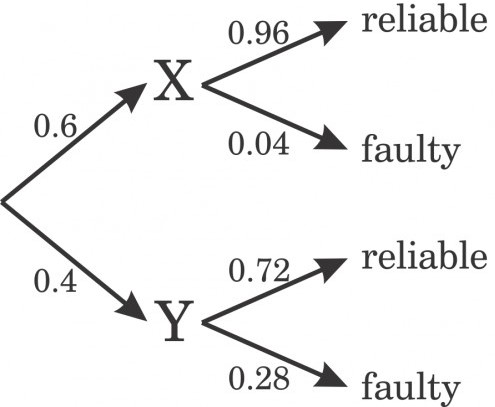
\includegraphics[width=0.5\textwidth]{solutions/cs/2012/63/Figures/A_4_1.png}
\end{center}
\end{figure}
Let Consider, Bernoulli random variables say $X,Y$ and $R$.
\begin{table}[h]
\resizebox{\columnwidth}{!}{
\begin{tabular}{|l|l|l|}
\hline
 & Refer to probability that product & Result \\ \hline
$Pr(X=1)$ & from supplier $X$ & $0.6$ \\ \hline
$Pr(Y=1)$ & from supplier $X$ & $0.4$ \\ \hline
$Pr(R=1)$ & is reliable &  \\ \hline
$Pr(R=0)$ & is faulty &  \\ \hline
$Pr(R=1/X=1)$ & from supplier $X$ is reliable & $0.96$ \\ \hline
$Pr(R=1/Y=1)$ & from supplier $Y$ is reliable & $0.72$ \\ \hline
\end{tabular}}
\caption{probability of random variables.}
\label{tab:my-table}
\end{table}
Required probability is $Pr(Y=1|R=1)$.So,
\begin{align}
&Pr(Y=1|R=1)=\frac{Pr(Y=1,R=1)}{Pr(R=1)}\\
&=\frac{Pr(Y=1)Pr(R=1/Y=1)}{Pr(X=1)Pr(R=1/X=1)+Pr(Y=1)P(R=1/Y=1)}\\
&=\frac{(0.4)(0.72)}{(0.6)(0.96)+(0.4)(0.72)}=0.334
\end{align}

%
\item A person who speaks truth $3$ out of $4$ times,throws a fair dice with six faces and informs the outcome is $5$.The probability that the outcome is really $5$ is
\\
\solution
Let $X \in \{0,1\}$ represent the random variable,where $0$ represents person speaking false,$1$ represents person speaking truth.\\
Let $Y \in \{1,2,3,4,5,6\}$  represent random variable,where $1,2,3,4,5,6$ represents person informs outcome of dice is $1,2,3,4,5,6$,respectively.\\
\begin{table}[h!]
\resizebox{\columnwidth}{!}
{ 
\begin{tabular}{|c|c|c|}
\hline
Event & definition & value\\
\hline
$ \pr{X=1} $ & Probability of person  & $\frac{3}{4}$\\
&speaking truth & \\
\hline
$ \pr{X=0} $ & Probability of person & $\frac{1}{4}$ \\
& speaking false & \\
\hline
$\pr{Y=5|X=1}$ & Probability of person  & \\
&  informing outcome is $5$ & $\frac{1}{6}$  \\
& if person speaks truth & \\
\hline
$\pr{Y=5|X=0}$ & Probability of person & \\
& informing outcome is $5$ &  $\frac{5}{6}$ \\
& if person speaks false & \\ 
\hline
\end{tabular}
}
\caption{Table 1} 
\label{xe2021-9:tab:1}
\end{table}
From Baye's theorem
\begin{align}
\pr{Y=5}&=\pr{Y=5|X=1} \times \pr{X=1} \notag \\
 & +\pr{Y=5|X=0} \times \pr{X=0}  \label{xe2021-9:1}
 \end{align}
Substiting values from table \eqref{xe2021-9:tab:1} in \eqref{xe2021-9:1}
\begin{align}
\pr{Y=5} &=\frac{8}{24} \label{xe2021-9:2} \\
\pr{(X=1)(Y=5)}&= \pr{Y=5|X=1} \notag \\
& \times \pr{X=1} \\ 
&= \frac{3}{24}  \label{xe2021-9:3}
\end{align}
We need to find $\pr{X=1|Y=5}$ \\
\begin{align}
\pr{X=1|Y=5} &= \frac{\pr{(X=1 ) (Y=5)}}{\pr{Y=5}} \\
&=\frac{3}{8}
\end{align}

%
\item  The probabilities that a student passes in Mathematics, Physics and Chemistry are m,p, and
c respectively. Of these subjects, the student has 75\% chance of passing in at least one, a
50\% chance of passing in at least two and a 40\% chance of passing in exactly two.
Following relations are drawn in m, p, c:
    \begin{enumerate}[label=(\Roman*)]
        \item p + m + c = 27/20
        \item p + m + c = 13/20
        \item (p)$\times$ (m) $\times$ (c) =1/10
    \end{enumerate}
    \begin{enumerate}[label=(\Alph*)]
      \item Only relation I is true
      \item Only relation II is true
      \item Relations II and III are true
      \item Relations I and III are true
    \end{enumerate}
%
\solution

Let M,P,C be the events representing student passes in Mathematics,Physics,Chemistry respectively.
\begin{align}
    \pr{M}&=m\\
    \pr{P}&=p\\
    \pr{C}&=c
\end{align}
The given information can be represented as
\begin{align}
    \pr{M+P+C}=75\%=\dfrac{3}{4}\label{atleast_1}\\
    \pr{MP+PC+CA}=50\%=\dfrac{1}{2}\label{atleast_2}\\
    \pr{MP+PC+CA-3MPC}=40\%=\dfrac{2}{5} \label{only_2}
\end{align}
\eqref{atleast_2} and \eqref{only_2} can also be written as
\begin{align}
    \pr{MP}+\pr{PC}+\pr{CM}&\nonumber\\-2\pr{MPC}&=\dfrac{1}{2}\\
    \pr{MP}+\pr{PC}+\pr{CM}&\nonumber\\-3\pr{MPC}&=\dfrac{2}{5}
\end{align}
Subtracting and solving the above two equations we get,
\begin{align}
    \pr{MPC}&=\dfrac{1}{10}\\
    \pr{MP}+\pr{PC}+\pr{CM}&=\dfrac{7}{10}
\end{align}
Using inclusion-exclusion principle, We can express \eqref{atleast_1} as
\begin{align}
\pr{M}+\pr{P}+\pr{C}&\nonumber\\
-[\pr{MP}+\pr{PC}+\pr{CM}]&\nonumber\\
      +\pr{MPC}&=\dfrac{3}{4}\\
    p+m+c-\dfrac{7}{10}+\dfrac{1}{10}&=\dfrac{3}{4}\\
    p+m+c&=\dfrac{27}{10}
\end{align}
There is no constant answer for the product of p,m,c which is shown in simulation.\\\\
\centering $\therefore$ Only relation I is true.

%
\item Let $X$ and $Y$ denote the sets consisting 2 and 20 distinct elements respectively and $F$ denote the set of all possible functions defined from $X$ and $Y$. Let $f$ be randomly chosen from $F$. The probability of f being one to one is :
\\
\solution
We know, every $x \in X$ can be mapped to one of 20 elements in $Y$.
\begin{align}
    n(F) = 20 \times 20 = 400
\end{align}

For one to one functions,  the first element in $X$ has 20 elements it can be mapped to, and second element in $X$ has only 19 elements.(to avoid repetition).
\begin{align}
    n(f) = 20 \times 19 = 380
\end{align}
Required probability:
\begin{align}
    \frac{n(f)}{n(F)} = \frac{380}{400} = \frac{19}{20}
\end{align}

%
\item The probability that a number selected at random between 100 and 999 (both inclusive) will not contain digit 7 is.
\solution

Let's assume a random 3-digit number be $xyz$.\\
Where $x,y,z$ are 3 random single-digit integers such that
\begin{align}
x\in \{1,2,3,4,5,6,7,8,9\}\\
y\in \{0,1,2,3,4,5,6,7,8,9\}\\
z\in \{0,1,2,3,4,5,6,7,8,9\}
\end{align}
\begin{enumerate}
\item
Probability of selecting $x$ without including 7
\begin{align}
    \Pr{(x\neq 7)}&=\frac{8}{9}
\end{align}
\item
Probability of selecting $y$ without including 7
\begin{align}
    \Pr{(y\neq 7)}&=\frac{9}{10}
\end{align}
\item
Probability of selecting $z$ without including 7
\begin{align}
    \Pr{(z\neq 7)}&=\frac{9}{10}
\end{align}
\end{enumerate}
So,the total probability of a random 3-digit number $xyz$ will not contain 7\\
\begin{align}
    &=\Pr{(x\neq 7)}\times\Pr{(y\neq 7)}\times\Pr{(z\neq 7)}\\
    &=\frac{8}{9}\times\frac{9}{10}\times\frac{9}{10}\\
    &=\frac{18}{25}
\end{align}
The probability of a number selected at random between 100 and 999 (both inclusive) will not contain digit 7 is $\frac{18}{25}$

%
\item A class of twelve children has two more boys than girls. A group of three children are randomly picked from this class to accompany the teacher on the field trip. What is the probability that the group accompanying the teacher contains more girls than boys.\\
\begin{enumerate}[label=(\alph*)]
\item $0$\\
\item $\frac{325}{864}$ \\
\item$\frac{525}{864}$\\
\item$\frac{5}{12}$
\end{enumerate}
\solution


Let $X \in \{0,3\}$ be a discrete random variable which denotes the number of girls in the group of 3.\\ 
Since, there are two more boys than girls:\\
\begin{align}
    \text{Total number of boys} (B) = 7  \notag \\
    \text{Total number of girls} (G) = 5  \notag\\
    \pr{X=c}=\frac{\comb{5}{c}\times \comb{7}{3-k}}{\comb{12}{3}} \label{ee2018-8:1.0.1}
\end{align}


For number of girls more than boys required probability = $ \pr{2\le X \le 3}$ and hence, following cases are possible. 
\begin{enumerate}
    \item X=3
    \begin{align}
        \pr{X=3} = \frac{\comb{5}{3}}{\comb{12}{3}}, \text{using \eqref{ee2018-8:1.0.1}} \notag
    \end{align}
    \item X=2
    \begin{align}
        \pr{X=2} = \frac{\comb{5}{2}\times\comb{7}{1}}{\comb{12}{3}}, \text{using \eqref{ee2018-8:1.0.1}} \notag
    \end{align}
\end{enumerate}
\begin{align}
   \text {So, required probability }=  \frac{\comb{5}{2}\times\comb{7}{1}}{\comb{12}{3}} + \frac{\comb{5}{3}}{\comb{12}{3}} = \frac{4}{11} \notag
\end{align}



%
\item Suppose that a shop has an equal number of LED bulbs of two different types. The probability of an LED bulb lasting more than 100 hours given that it is of Type 1 is 0.7, and given that it is of Type 2 is 0.4. The probability that an LED bulb chosen uniformly at random lasts more than 100 hours is
\\
\solution 

Let the random variable $X\in\{1,2\}$ represent the type of the chosen bulb. $X=1$ denotes a Type 1 bulb, while $X=2$ denotes a Type 2 bulb. Given,
\begin{align}
\tag{5.1}
    n(X=1)=n(X=2)\\
\tag{5.2}\Rightarrow p_{X}(1)=p_{X}(2)=\dfrac{1}{2}
\end{align}
Let the random variable $Y\in\{0,1\}$ represent if a bulb lasts more than 100 hours. $Y=1$ denotes that it lasts, while $Y=0$ denotes that it doesn't. Given, 
\begin{align}
\tag{5.3}
    p_{Y|X}(1|1)=0.7\\
\tag{5.4}
    p_{Y|X}(1|2)=0.4
\end{align}
To find : $p_{Y}(1)$
\begin{align}
\tag{5.5}
p_{Y}(1)&=p_{Y|X}(1|1)p_{X}(1)+p_{Y|X}(1|2)p_{X}(2)\\
\tag{5.6}
&p_{Y}(1)=(0.7)(0.5)+(0.4)(0.5)\\
\tag{5.7}
&\therefore p_{Y}(1)=0.55
\end{align}

%
\item The probability that a given positive integer lying between 1 and 100 ( both inclusive) and is NOT divisible by 2 or 3 or 5 is \dots
\\
\solution
Let $A,B,C$ are events where a positive integer between 1 and 100 ( both inclusive ) is divisible by 2, 3, 5 respectively.
\begin{align}
  \Pr(A) &= \frac{1}{2}\\
  \Pr(B) &= \frac{33}{100} \\
  \Pr(C) &= \frac{1}{5} \\
  \Pr(AB) &= \frac{16}{100} \\
  \Pr(BC) &= \frac{6}{100} \\
  \Pr(AC) &= \frac{1}{10} \\
  \Pr(ABC) &= \frac{3}{100} 
\end{align}
Required probability : $\Pr(A+B+C)^{\prime}$
\begin{multline}
\Pr(A+B+C)^{\prime}  = 1-\Pr(A+B+C) \\  
 = 1-\Pr(A)-\Pr(B)-\Pr(C)+{}\\ \Pr(AB) + \Pr(BC)+ \Pr(AC){}\\
 -\Pr(ABC) 
    = 0.26 
\end{multline}

%
\item What is the probability that a divisor of $10^{99}$ is a multiple of $10^{96}$ ?
\vspace{0.5 cm}
(A) $\dfrac{1}{625}$ \hspace{0.5 cm} (B) $\dfrac{4}{625}$ \hspace{0.5 cm} (C) $\dfrac{12}{625}$ \hspace{0.5 cm} (D) $\dfrac{16}{625}$
%
\\
\solution
Let 
\begin{align*}
& X= \{ (x,y) : 0\leq x \leq 99 ,0\leq y \leq 99 \}
\end{align*} 
be a set of random variables, $N=2^x5^y$ , 
\begin{align}
& \implies \forall (x,y) \in X, \text{ N is a divisor of } 10^{99}\\
&\implies n (X) = 100\times 100=10^4 \label{cs2010-27:eq_1}
\end{align}
Let 
\begin{align*}
&Y=\{(x,y) : (x,y)\in X , x \geq 96,y\geq 96\}\\
&N_1= 2^x5^y 
\end{align*}
\begin{align}
&\implies \forall (x,y) \in  Y ,N_1 | 10^{99} \text{ and is multiple of } 10^{96} \\
&\implies n(Y)=4\times 4=16 \label{cs2010-27:eq_2}
\end{align}
Let P denotes the probability that a divisor of $10^{99}$ is a multiple of $10^{96}$ then
$$P=\dfrac{n(Y)}{n(X)}$$
From \ref{cs2010-27:eq_1} and \ref{cs2010-27:eq_2} we can write
$$P=\dfrac{16}{10^4}=\dfrac{1}{625}$$
So the probability is $\dfrac{1}{625}$, option (\textbf{A}).

%
\item There are five bags each containing identical sets of ten distinct chocolates. One chocolate is picked from each bag.\\
The probability that atleast two chocolates are identical is?\\
\solution

Let random variable $X\in\{0,2,3,4,5\}$ denote the maximum number of identical chocolates picked in an experiment.
\begin{align}
    P\brak{X\geq2} &= 1-P\brak{X=0}\\
    &=1-\frac{10\times9\times8\times7\times6}{10^{5}}\\
    &=1-0.3024\\
    &=0.6976
\end{align}


%
\item Raju has four fair coins and one fair dice. At first Raju tosses a coin. If the coin shows head then he rolls the dice and the number that dice shows is taken as his score. If the coin shows tail then he tosses three more coins and the total number of tails shown (including the first one) is taken as his score. If Raju tells that his score is 2 then the probability that he rolled the dice is (up to two decimal places):
%
\\
\solution
Let $X_i$ denote the random variable function for the $i$th coin $i\in\{1,2,3,4\}$.\\
$X_i\in(0,1)$ where 0 represents head and 1 represents tail $i\in\{1,2,3,4\}$.
\\[5pt]
\begin{tabular}{|c|c|c|}
\hline
     &Head&Tail  \\
     \hline
     $X_i=k$&0&1\\
     \hline
\end{tabular}
\begin{equation}\label{ec29-1:coin}
\Pr(X_i=k)=\dfrac{1}{2} 
\end{equation}
$k\in\{0,1\}$ and $i\in\{1,2,3,4\}$.
\\
Let $Y$ denote the random variable function for the dice.\\
$Y\in(1,2,3,4,5,6)$ where 1 represents dice showing 1 and so on.
\\[5pt]
\begin{tabular}{|c|c|c|c|c|c|c|}
\hline
     Dice number&1&2&3&4&5&6  \\
     \hline
     $Y=k$&1&2&3&4&5&6\\
     \hline
\end{tabular}
\\
\begin{equation}\label{ec29-1:dice}
\Pr(Y=k)=\dfrac{1}{6} 
\end{equation}
$k\in\{1,2,3,4,5,6\}$.
\\[20pt]
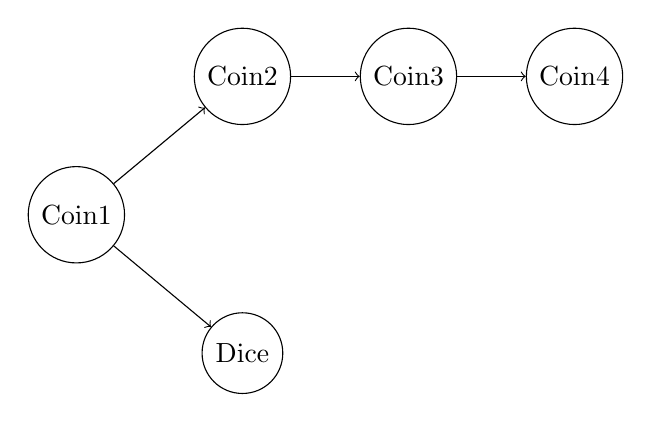
\begin{tikzpicture}
      [sibling distance=10em,level distance=6em, grow=right,
      every node/.style={shape=circle,draw,align=center},->]
      \node{Coin1}
   child
   {
    node{Dice}
   }
   child
   {
    node{Coin2}
      child
      {
        node{Coin3}
        child
      {
        node{Coin4}
      }
      }
    };
\end{tikzpicture}
Let B denote the event that out of last three coins, only one shows tail. \\
By Binomial Distribution,
\begin{align}
\Pr(B)&=\comb{3}{1}\brak{{\dfrac{1}{2}}}^3
\\[\parskip]
&=\dfrac{3}{8}
\end{align}
%
Since tossing a coin and rolling a dice are independent events,
\begin{equation}\label{ec29-1:independent theorem}
\Pr( (X_i=k),(Y=l) )= \Pr(X_i=k)\cdot \Pr(Y=l)
\end{equation}
$k\in\{0,1\}$ and $l\in\{1,2,3,4,5,6\}$.

Let A denote the event that the score is 2.

Clearly,
\begin{align}
\Pr(A)\nonumber&=\Pr(Y=2|X_1=0)\cdot \Pr(X_1=0) \\
    &+ \Pr(B|X_1=1)\cdot \Pr(X_1=1) 
\\[\parskip]
&=\Pr( (X_1=0),(Y=2) ) + \Pr( (X_1=1), B)
\\[\parskip]
&=\Pr(X_1=0)\cdot \Pr(Y=2)+ \Pr(X_1=1) \cdot \Pr(B)
\\[\parskip]
&=\dfrac{13}{48}
\end{align}
We have to find $\Pr(X_1=0|A)$
\begin{align}
\Pr(X_1=0|A)&=\dfrac{\Pr(A,(X_1=0) )}{\Pr(A)}
\\[\parskip]
&=\dfrac{\Pr(X_1=0)\cdot \Pr(Y=2)}{\Pr(A)}
\\[\parskip]
&=0.31
\end{align}

\textbf{Therefore, required probability = 0.31}



%
\item A bag contains 10 white balls and 15 black balls . Two balls are drawn in succession. The probability that one of them is white and the other is black is.
\\
\solution

Let X denote the number of white balls in the first draw and Y be the number of white balls in second draw and let E be the event mentioned in question.
\begin{multline}
\Pr(E) = \Pr(X=1)\times \Pr(Y=0/X=1) \\
+ \Pr(X=0)\times \Pr(Y=1/X=0)
\end{multline}
Let m and n be the number of black and white balls in the box.
\begin{align}
&\Pr(X=0) = \frac{m}{m+n} \\ 
&\Pr(X=1)=\frac{n}{m+n}\\
&\Pr(Y=0/X=0)=\frac{m-1}{m+n-1}\\
&\Pr(Y=1/X=0)=\frac{n}{m+n-1}\\
&\Pr(Y=0/X=1)=\frac{m}{m+n-1}\\
&\Pr(Y=1/X=1)=\frac{n-1}{m+n-1}
\end{align}
\begin{multline}
\Pr(E)=\frac{n}{m+n}\times \frac{m}{m+n-1}\\
+\frac{m}{m+n}\times\frac{n}{m+n-1}=\frac{1}{2}
\end{multline}

%
\item The box 1 contains chips numbered 3, 6, 9, 12 and 15. The box 2 contains chips numbered 6, 11, 16, 21 and 26.
Two chips, one from each box are drawn at random. The numbers written on these chips are multiplied. The probability 
for the product to be an even number is
%
\begin{enumerate}
\item $\frac{6}{25}$
\item $\frac{2}{5}$
\item $\frac{3}{5}$
\item $\frac{19}{25}$
\end{enumerate}
%
\solution
Consider two independent random variables X and Y which denotes the number on the chip drawn from box 1 and box 2 respectively.\\
X can take the values 3, 6, 9, 12, 15\\
X can take the values 6, 11, 16, 21, 26
\begin{align}
\Pr\brak{X\times Y=even}\notag\\
=&\Pr\brak{X=even,Y=odd}\notag\\&+\Pr\brak{X=odd,Y=even}\notag\\&+\Pr\brak{X=even,Y=even}\\
=&\frac{2}{5}\times\frac{2}{5}+\frac{3}{5}\times\frac{3}{5}+\frac{2}{5}\times\frac{3}{5}\\
=&\frac{19}{25}
\end{align}
%
\item A box contains 25 parts of which 10 are defective. Two parts are being drawn simultaenously in a random manner from the box. The probability of both parts being good is\\
$(A)\frac{7}{20}\ \ \ (B)\frac{42}{125}\ \ \ (C)\frac{25}{29}\ \ \ (D)\frac{5}{9}$
%
\solution
%
Let $X_1,X_2\in\{0,1\}$ represent the parts, where $0$ represents good part, $1$ represent defective part. From the given information
\begin{align}
\pr{X_1=0}=\frac{15}{25}=\frac{3}{5}\\
\pr{X_2=0|X_1=0}=\frac{14}{24}=\frac{7}{12}
\end{align}
Then,
\begin{multline}
\pr{X_1=0,X_2=0}\\
=\pr{X_2=0|X_1=0}\times \pr{X_1=0}=\frac{7}{20}
\end{multline}
%
\item From a pack of regular playing cards, two cards are drawn at random. What is
the probability that both cards will be Kings, if the first card is NOT replaced?
    \begin{enumerate}
    \item $\frac{1}{26}$
    \item $\frac{1}{52}$
    \item $\frac{1}{169}$
    \item $\frac{1}{221}$
\end{enumerate}
%
\solution

Let $A,B \in \{0,1\}$, where $1$ denotes that card is a King, and $0$ denotes that card is not a King. $A$ denotes the first card is picked, $B$ denotes second card is picked.
\begin{align}
    \pr{A=1} &= \frac{4}{52}\\
    \pr{B=1|A=1} &=\frac{3}{51}
\end{align}
Applying Bayes Theorem, we need to find the value of $\pr{A=1,B=1}$:
\begin{align}
    &= \pr{B=1|A=1}\cdot \pr{A=1}\\
    &=\frac{4}{52} \cdot \frac{3}{51}\\
    &= \frac{1}{221}
\end{align}
The Probability that both cards are king is $\frac{1}{221}$, Hence \textbf{Option 4 }is correct

%
\item A group consists of equal number of men and women. Of this group, 20\% of the men and 50\% of the women are unemployed. If a person is selected at random from this group, the probability of the selected person being employed is  
%
\solution

Let the random variable $X\in\{0,1\}$ represent the gender of the person. $X=0$ denotes a female, while $X=1$ denotes a male. Given,
\begin{align}
\tag{4.1}
    n(X=0)=n(X=1)\\
\tag{4.2}\Rightarrow p_{X}(0)=p_{X}(1)=\dfrac{1}{2}
\end{align}
Let the random variable $Y\in\{0,1\}$ represent if the person is employed. $Y=0$ denotes unemployed, while $Y=1$ denotes employed. Given, 
\begin{align}
\tag{4.3}
    p_{Y|X}(0|0)=0.5\Rightarrow p_{Y|X}(1|0)=0.5\\
\tag{4.4}
    p_{Y|X}(0|1)=0.2\Rightarrow p_{Y|X}(1|1)=0.8
\end{align}
To find : $p_{Y}(1)$
\begin{align}
\tag{4.5}
p_{Y}(1)&=p_{Y|X}(1|0)p_{X}(0)+p_{Y|X}(1|1)p_{X}(1)\\
\tag{4.6}
&p_{Y}(1)=(0.5)(0.5)+(0.8)(0.5)\\
\tag{4.7}
&\therefore p_{Y}(1)=0.65
\end{align}
%

%
\item The probability that a student knows the correct answer to a multiple choice question is $\frac{2}{3}$. If the student does not know the answer, then the student guesses the answer. The probability of the guessed answer being correct is $\frac{1}{4}$. Given that the student has answered the question correctly, the conditional probability that the student knows the correct answer is

    \begin{enumerate}
        \item $\frac{2}{3}$
        \item $\frac{3}{4}$
        \item $\frac{5}{6}$
        \item $\frac{8}{9}$
    \end{enumerate}
%
\solution


Let the following random variables and their values denote:
\begin{align*}
    A:\text{Knows correct answer} &= 1\\
    B:\text{Marks correct answer} &= 1
\end{align*}
\begin{align}
    \therefore \pr{A=1} &= \frac{2}{3}\\
    \pr{B =1|A=1} &= 1\\
    \pr{B =1|A=0} &= \frac{1}{4}
\end{align}
Applying Bayes Theorem, the value of $\pr{B = 1}$ is :
\begin{align}
\nonumber
    \pr{B = 1} &= \pr{B =1|A=1}\pr{A=1}\\ 
    &\quad+\pr{B =1|A=0}\pr{A=0}\\
    &= 1\cdot \frac{2}{3} + \frac{1}{4}\cdot \frac{1}{3}  =\frac{3}{4} \label{me2013-45:pr_denom}
\end{align}
Applying Bayes Theorem, calculating the value of $\pr{B =1, A=1}$ is:
\begin{align}
    &=\pr{B =1|A=1}\pr{A=1}\\
    &=1\cdot \frac{2}{3} \label{me2013-45:pr_num}
\end{align}
Applying Bayes Theorem, we need to find the value of $\pr{A=1|B =1}$. Upon substituting from \eqref{me2013-45:pr_num} and \eqref{me2013-45:pr_denom}, we get
\begin{align}
    &= \frac{\pr{B =1, A=1}}{\pr{B = 1}}\\
    &= \frac{8}{9}
\end{align}
The correct answer is \textbf{Option 4}.

%
\item Consider an unbiased cubic dice with opposite faces coloured identically and each face coloured red, blue or green such that each colour appears only two times on the dice. If the dice is thrown thrice, the probability of obtaining red colour on top face of the dice at least twice is $\rule{1.6cm}{0.15mm}$ .
%
\solution

Let $X \in \{ 0, 1, 2, 3\}$ be the random variable representing the number of times a red face is obtained. Then $X$ is a binomial distributions with parameter:
\begin{align}
    p &= \frac{\text{number of red coloured faces}}{\text{total number of faces}}
    \\ &= \frac{2}{6}
    \\ &= \frac{1}{3}
\end{align}
Then,
\begin{align}
    \Pr(X=i) &= 
	\begin{cases}
	\comb{3}{i}(p)^i(1-p)^{3-i} &  i \in \{0, 1, 2, 3\}\\ 
	0 & \text{otherwise}
	\end{cases}
	\\ &= 
	\begin{cases}
	\comb{3}{i}(\frac{1}{3})^i(1-\frac{1}{3})^{3-i}  &  i \in \{0, 1, 2, 3\}\\ 
	0 & \text{otherwise}
	\end{cases}
    \\F_X(i) &= 
	\begin{cases}
	\sum_{k=0}^i\comb{3}{k}(p)^k(1-p)^{3-k} &  i \in \{0, 1, 2, 3\}\\ 
	0 & \text{otherwise}
	\end{cases}
\end{align}
\begin{align}
    \Pr{(X \geq 2)} &= \Pr{(X=2)} + \Pr{(X=3)}
    \\&= \frac{6}{27} + \frac{1}{27}
    \\&= \frac{7}{27}
\end{align}


\item  The chance of a student passing an exam is 20\%. The chance of a student passing the exam and getting above 90\% marks is 5\%. GIVEN that a student passes the examination, the probability that the student gets above 90\% marks is
%
\\
\solution
\begin{table}[h]
\setlength{\tabcolsep}{40pt}
    \begin{tabular}{c c}
         a). $\cfrac{1}{18}$ & c). $\cfrac{1}{4}$ \\
         b). $\cfrac{2}{9}$  & d). $\cfrac{5}{18}$
    \end{tabular}
\end{table}

Let A be the event that the student passes the exam and B be the event that the student gets above 90\% in the exam. Thus we need to find \pr{B|A}. We are given
\begin{align}
    \pr{A}  &= \cfrac{1}{5}\\
    \pr{AB} &= \cfrac{1}{20}
\end{align}
Thus required probability 
\begin{align}
    &= \pr{B|A}\\
    &= \cfrac{\pr{AB}}{\pr{A}}\\
    &= \cfrac{1}{4}    
\end{align}
Thus option B is the correct option.

\item Four red balls, four green balls and four blue balls are put in a box. Three balls are pulled out of the box at random one after another without replacement. The probability that all the three balls are red is  
%
\\
\solution
 

Let $A,B,C \in \{0,1\}$, where $0$ denotes that pulled out ball is red, and $1$ denotes that pulled out ball is not red. $A$ denotes the first ball is pulled out of the box,$B$ denotes the second ball is pulled out of the box,$C$ denotes the third ball is pulled out of the box.
\begin{align}
    \pr{A=0} &= \frac{4}{12} \label{me2018-1:a}\\
    \pr{B=0|A=0} &=\frac{3}{11} \label{me2018-1:b}\\
    \pr{C=0|(B=0,A=0)} &=\frac{2}{10}  \label{me2018-1:c}
\end{align}
Applying Bayes Theorem to $\pr{A=0,B=0}$,
\begin{align}
  \pr{A=0,B=0}  &= \pr{B=0|A=0}\pr{A=0}
  \end{align}
  using \eqref{me2018-1:a} and \eqref{me2018-1:b} ,
\begin{align}  
    &=\frac{3}{11}\cdot \frac{4}{12}\\
    &= \frac{1}{11}  \label{me2018-1:d}
\end{align}
similarly $\pr{A=0,B=0,C=0}$ can be written as, 
\begin{align}
  &= \pr{C=0|(B=0,A=0)}\pr{A=0,B=0}
  \end{align}
  using \eqref{me2018-1:c} and \eqref{me2018-1:d} , 
  \begin{align}
    &=\frac{2}{10}\cdot \frac{1}{11}\\
    &= \frac{1}{55}
\end{align}
%
\item Consider a company that assembles computers.The probability of a faulty assembly of any computer is p.The company therefore subjects each computer to testing process.This testing process gives the correct result for any computer with a probability of q.What is the probability of a computer being declared faulty?
\begin{enumerate}
\item pq+(1-p)(1-q)
\item (1-q)p
\item (1-p)q
\item pq
\end{enumerate}
%
\solution

Let $X_i \in \cbrak{0,1}$ where $\pr{X_1 = 1}$ represents the computer is faulty before testing, $\pr{X_2 = 1}$ represents the testing process gives the correct result.
\begin{table}[h]
\centering 
\caption{}
\begin{tabular}{|c|c|c|}
\hline
           & $X_1 = 0$  & $X_1 = 1$\\
\hline
$X_2 = 0$  & (1-p)(1-q) & (1-q)p \\
\hline
$X_2 = 1$  &  (1-p)q    &  pq \\
\hline
\end{tabular}
\label{cs2010-26:table:}
\end{table}
 
Table \ref{cs2010-26:table:} represents the probabilities of all possible cases.The probability of a computer being declared as faulty is 
\begin{align}
\tag{1.1}
     &= \pr{(X_2 = 1)(X_1 = 1)}+\pr{(X_2 = 0)(X_1 = 0)}\\
\tag{1.2}
     &= pq+(1-p)(1-q) 
\end{align}
The required option is (A).

%
\item  An array of 25 distinct elements is to be sorted using quicksort. Assume that the pivot element is chosen uniformly at random. The probability that the pivot element gets placed in the worst possible location in the first round of partitioning (rounded off to 2 decimal places) is ----
%
\solution

The worst possible place, the pivot element can be placed is at extreme left or extreme right. So, there are only 2 worst possible locations. \\
\begin{equation}
   Pr (X1\ is\ compared\ to\ Xn) = \dfrac{2}{n}.
\end{equation}
Total number of pivot elements = 25. \\
Number of worst possible location of pivot element gets placed after first round of partitioning = 2. \\
Probability of placing pivot element in worst possible locations = $\dfrac{2}{25}$ = 0.08. 

Maximum,
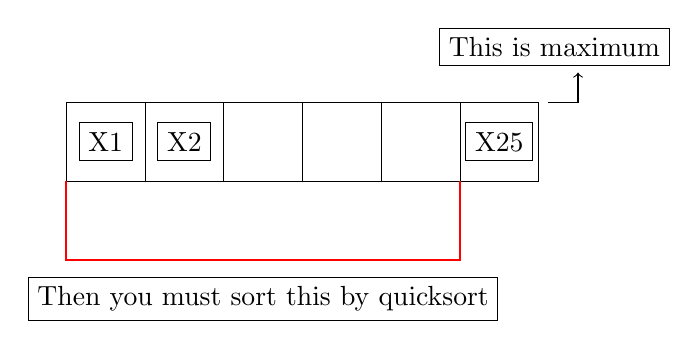
\begin{tikzpicture}
\draw[step=1cm,black,very thin] (0,0) grid (6,1)  node[anchor=north west] {};
\node[draw] at (0.5,0.5) {X1};
\node[draw] at (1.5,0.5) {X2};
\node[draw] at (5.5,0.5) {X25};
\node[draw] at (6.2,1.7) {This is maximum};
\node[draw] at (2.5,-1.5) {Then you must sort this by quicksort};
\node (A) at (6, 1) {};
\node (B) at (6.5, 1.5) {};
\draw[->, to path={-| (\tikztotarget)}]
  (A) edge (B) ;
\draw[red,thick,solid] (0,0) -- (0,-1) -- (5,-1) -- (5,0);
\end{tikzpicture} 
Minimum, \\ 
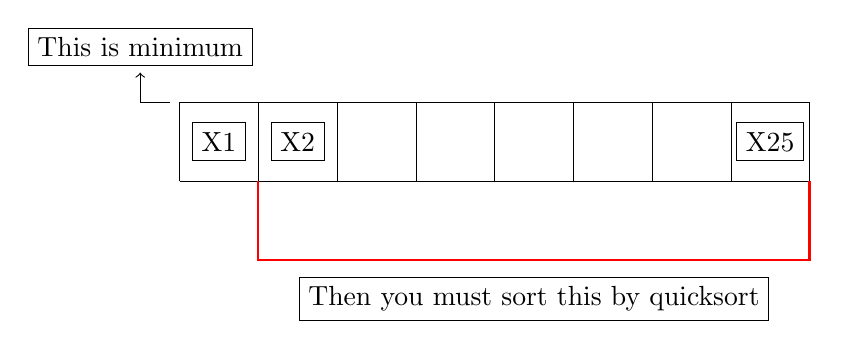
\begin{tikzpicture}
\draw[step=1cm,black,very thin] (0,0) grid (8,1)  node[anchor=north west] {};
\node[draw] at (0.5,0.5) {X1};
\node[draw] at (1.5,0.5) {X2};
\node[draw] at (7.5,0.5) {X25};
\node[draw] at (-0.5,1.7) {This is minimum};
\node[draw] at (4.5,-1.5) {Then you must sort this by quicksort};
\node (A) at (0, 1) {};
\node (B) at (-0.5, 1.5) {};
\draw[->, to path={-| (\tikztotarget)}]
  (A) edge (B) ;
\draw[red,thick,solid] (1,0) -- (1,-1) -- (8,-1) -- (8,0);
\end{tikzpicture}


%
\item  There are 3 red socks, 4 green socks and 3 blue socks. You choose 2 socks. The probability that they are of the same colour is 

\begin{enumerate}
    \item $\frac{1}{5}$
    \item $\frac{7}{30}$
    \item $\frac{1}{4}$ 
    \item $\frac{4}{15}$ 
\end{enumerate}
%
\solution
Let $X_1 \in \{0,1,2\}$ and $X_2 \in \{0,1,2\}$ be two Random Variables representing the colour of socks taken in $1^{st}$ draw and in $2^{nd}$ draw respectively.
$X_1 = 0$, $X_1 = 1$, $X_1 = 2$ represent choosing Red, Green, Blue socks in the first draw respectively.
Similarly, $X_2 = 0$, $X_2 = 1$, $X_2 = 2$ represent choosing Red, Green, Blue socks in the second draw respectively.
Now, the probability that the socks drawn in $1^{st}$ draw and $2^{nd}$ draw are of the same colour is given by
\begin{align*}
\pr{X_1 = X_2}    
\end{align*}
Now,
\begin{align}
\pr{X_1 = X_2} &= \sum_{k = 0}^{k = 2} \pr{X_1 = X_2 = k} \\
&= \sum_{k = 0}^{k = 2} \pr{X_1 = k, X_2 = k} \\
&= \sum_{k = 0}^{k = 2} \pr{X_1 = k} \pr{(X_2 = k) | (X_1 = k)}
\end{align}
\begin{align}
&= \pr{X_1 = 0} \pr{(X_2 = 0) | (X_1 = 0)} \\ \nonumber
& \quad + \pr{X_1 = 1} \pr{(X_2 = 1) | (X_1 = 1)} \\ \nonumber
& \quad + \pr{X_1 = 2} \pr{(X_2 = 2) | (X_1 = 2)}
\end{align}
From the given information in the question,
\begin{align}
\pr{X_1 = X_2} &= \left(\frac{3}{10} \right) \left(\frac{2}{9} \right) + \left(\frac{4}{10} \right) \left(\frac{3}{9} \right) + \left(\frac{3}{10} \right) \left(\frac{2}{9} \right) \\
&= \left(\frac{6}{90} \right) + \left(\frac{12}{90} \right) + \left(\frac{6}{90} \right) \\
&= \frac{24}{90} = \frac{4}{15}
\end{align}
Therefore, the probability that the two socks are of same colour is $\frac{4}{15}$.
Hence, the correct option is 4) $\frac{4}{15}$.


%
\item Suppose we uniformly and randomly select a permutation from the 20\(!\) permutations of 1,2,3,\ldots,20. What is the probability that 2 appears at an earlier position than any other even number in the selected permutation.
\begin{enumerate}[label=(\Alph*)]
    \item \(\displaystyle\frac{1}{2}\)\newline
    \item \(\displaystyle\frac{1}{10}\)\newline
    \item \(\displaystyle\frac{9!}{20!}\)\newline
    \item \normalsize{None of the above.}\newline
\end{enumerate}

%
\solution
 \begin{table}[ht]
  \centering
  \begin{tabular}{|c|c|}
        \hline
         Number of dices & \(n\) = 2\\
         \hline
         The total no. of outcomes & 36\\ 
        \hline
         Probability of 6 facing-up & \(p\) = 1/6 \\
        \hline
         Probability of 6 'NOT' facing-up & \(q\) = 5/6 \\
        \hline
         Number of sixes in the outcome & \(X\) \\ 
        \hline
    \end{tabular}
\end{table}
Probability of at least one six facing up
    \begin{align}
         & = {Pr(X = 1)} + {Pr(X = 2)} \\
         & = {^2 C _1}{p}{q} + {^2 C _2}{p^2}{q^0}\\
         & = {^2 C _1} \left( {\frac{1}{6}}\right) \left( {\frac{5}{6}}\right) + {^2 C _2} \left(\frac{1}{6}\right) ^2\\ 
         & = 2 \left(\frac{5}{36}\right) + \frac{1}{36}\\
         & = \frac{11}{36}
    \end{align}


\item Aishwarya studies either computer science or mathematics everyday. If she studies computer science on a day, then the probability she studies mathematics the next day is 0.6. If she studies mathematics on a day, then the probability she studies computer science the next day is 0.4.
Given that Aishwarya studies computer science on Monday, what is the probablity she studies computer science on Wednesday?
\begin{enumerate}[label=(\Alph*)]

%\setlength\itemsep{2em}
\item 0.24
\item 0.36
\item 0.4
\item 0.6

\end{enumerate}
%
\solution
Consider the following parameters
\begin{table}[h!]
    \begin{tabular}[width=\columnwidth]{|c|m{2.4cm}|m{3.1cm}|}
         \hline
        \textbf{Parameter\hspace{-1mm}}&\textbf{Definition}&\textbf{Value}\\
        \hline    
         S&State space (i.e possible states she can be in.)& $S=\{1,2\}$, where $1$ and $2$ represents her studying CS or maths respectively on that day.\\
         \hline
         {$\{X_0, X_1, \dots\}$}& \multicolumn{2}{p{5.8cm}|}{Random variables(which form a markov chain) where $X_i \in S$ represents her studying CS or maths on the $i$th day(i=0 for Monday)}\\
         \hline
         P& {The one \nolinebreak step state \nolinebreak transition  matrix (The elements $p_{ij}\nolinebreak=\nolinebreak\text{Pr}(X_{n+1}$ $= j\, |\, X_{n}=i)$ )}& {\vspace{-4mm}\begin{align}
        \hspace{3em}\,\,\,\,\overbrace{
         \begin{matrix}
        1 & \,\,\,2
        \end{matrix}}^{X_{n+1}}\nonumber
        \end{align}
        \vspace{-1cm}
        \begin{align}
        P=\,\scriptstyle{X_n}\, \bigg\{ \,\begin{matrix} 1\\ 2\end{matrix}\,
        \begin{bmatrix}
        x & \hspace{-3mm}0.6 \\
        0.4 & \hspace{-3mm}y 
        \end{bmatrix}
    	\label{transition_matrix}
        \end{align}}\\
         \hline
    \end{tabular}
    \label{cs2008-27:Parameters}
\end{table}
%%Consider the state space $S=\{1,2\}$, where $1$ represents Aishwarya studying CS and $2$ represents her studying maths on a particular day.\\ 
%%Let \{$X_0, X_1, \dots$ \} be a series of random variables. So we have the Markov chain  
%%\begin{align}
%%\{X_n\,|\, X_n \in S, n \geq 0\},
%%\end{align}% , where $X_n$ represents her studying CS or mathematics on the $n$th day. 
%%with initial distribution $\alpha = (\alpha_1 , \alpha_2) =(1,0)$ ($\because\alpha_i = \pr{X_0=i}$).\\
%%The state transition matrix $P=(p_{ij})$ for the markov chain (where $p_{ij}=\pr{X_{n+1}=j\, |\, X_{n}=i}$) is :-
%%\begin{align}
%%\hspace{3.3em}\overbrace{
%% \begin{matrix}
%%1 & \,\,\,\,\,\,2
%%\end{matrix}\nonumber}^{X_{n+1}}\nonumber
%%\end{align}
%%\vspace{-1cm}
%%\begin{align}
%%P\,\,=\,\,\,\,\scriptstyle{X_n\,\,} \bigg\{ \, \begin{matrix} 1\\ %%2\end{matrix}\,\,\,
%% \begin{bmatrix}
%%x & 0.6 \\
%%0.4 & y 
%%\end{bmatrix}\hspace{0.6cm}
%%\end{align}
\par As $X_n=0 \text{ and } X_n=1$ are mutually exclusive, we can easily calculate $x$ and $y$.
\begin{align}
   x=\pr{X_{n+1} = 0 |\, X_{n}=0} &= 1-\pr{X_{n+1} = 1 \,| X_{n}=0}\nonumber
    \\&= 0.4 \label{cs2008-27:x}\\
    y=\pr{X_{n+1} = 1 |\, X_{n}=1} &= 1-\pr{X_{n+1} = 0 \,| X_{n}=1}\nonumber
    \\&= 0.6 \label{cs2008-27:y}
\end{align}
\begin{figure}[h]
    \centering
     \begin{tikzpicture}[
roundnode/.style={circle, draw=black!90, fill=black!7, very thick, minimum size=7mm},
]
%Nodes
\node[roundnode]        (Computer_Science)        {1};
\node[roundnode]        (Mathematics)       [right=4cm of Computer_Science] {2};
%Lines
 \draw[every loop,
        auto=right,
        line width=0.7mm,
        >=latex,
        draw=orange,
        fill=orange]
            (Computer_Science) edge[bend right, auto=left]  node {0.6} (Mathematics)
            (Mathematics) edge[bend right, auto=right] node {0.4} (Computer_Science)
            (Computer_Science) edge[loop above]             node {0.4} (Computer_Science)
            (Mathematics) edge[loop above]             node {0.6} (Mathematics);
\end{tikzpicture}
    \par{Markov Diagram}
\end{figure}
\par Given that her initial state is $X_0=1$ ($\because$ she studies CS on Monday(n=0)).\\ The $\pr{X_{n+t}=j \, |\, X_{n}=i}$ is given by the $(i,j)$th position of $P^{\,t}$. Therefore $\pr{X_{2}=1 | X_{0}=1}$ ($\because$ n=2 for Wednesday) is the $(1,1)$th position of $P^2$.
\begin{align}
    P^2=\begin{bmatrix}
0.4 & 0.6 \\
0.4 & 0.6
\end{bmatrix}\times
\begin{bmatrix}
0.4 & 0.6 \\
0.4 & 0.6 
\end{bmatrix}=
\begin{bmatrix}
0.4 & 0.6 \\
0.4 & 0.6 
\end{bmatrix}
\end{align}
\par $\therefore$ The probability she studies computer science on Wednesday is $P_{1\,1}^{\,2} = 0.4$.\\
(\textbf{Ans: Option (C)})


%
\item  The probability that the top and bottom cards of a randomly shuffled deck are both aces is
\begin{description}
\item[$\brak{A}$]$\dfrac{4}{52}\times\dfrac{4}{52}$ \\
\item[$\brak{B}$]$\dfrac{4}{52}\times\dfrac{3}{52}$ \\
\item[$\brak{C}$]$\dfrac{4}{52}\times\dfrac{3}{51}$ \\
\item[$\brak{D}$]$\dfrac{4}{52}\times\dfrac{4}{51}$ \\
\end{description}
%
\solution

Let the following random variables and their values denote:
\begin{align*}
    A : \text{Top card is an ace} &= 1\\
    B : \text{Bottom card is an ace} &=1
\end{align*}
\begin{align}
    \pr{A=1} &= \frac{4}{52} \label{cs1996-32:eq1} \\
    \pr{B = 1|A = 1} &= \frac{3}{51} \label{cs1996-32:eq2}
\end{align}
Applying Bayes Theorem, 
\begin{align}
    \pr{B = 1, A = 1} &= \pr{B = 1|A = 1} \pr{A = 1}\\
\intertext{from \eqref{cs1996-32:eq1} and \eqref{cs1996-32:eq2},}
    \pr{B = 1, A = 1} &=   \frac{4}{52} \times\frac{3}{51}
\end{align}
\\The correct option is \textbf{Option (C)}.


%
\item Suppose a fair six-sided die is rolled once. If the value on the die is 1,2, or 3, the die is rolled a second time. What is the probability that the sum total of values that turn up is at least 6?
\begin{enumerate}
    \item 10/21
    \item 5/12
    \item 2/3
    \item 1/6
\end{enumerate}
%
\solution

Let us define a random variable $X \in \cbrak{0,1}$\\
\begin{table}[ht]
    \centering
    \begin{tabular}{|c|c|}
    \hline
    X=0 & Getting 1,2, or 3 on first roll\\
    \hline
    X=1 & Getting the sum total of values at least 6\\
    \hline
    \end{tabular}
    \caption{Random Variables}
    \label{cs2012-33:tab:Random Variables}
\end{table}

Probability of getting 1,2, or 3 on first roll is given by,
\begin{align}
    \pr{X=0}&=\cfrac{3}{6}= \cfrac{1}{2}\\
\end{align}
Probability of getting sum total of 6 on first roll is given by,
\begin{align}   
    \pr{X=1}&= \cfrac{1}{6}\\
\end{align} 
Probability of getting sum total of 6 after getting 1,2,or,3 in first roll is given by,
\begin{align}    
    \pr{X=1|X=0}&=\cfrac{9}{18}= \cfrac{1}{2}
\end{align}
Now,probability of getting sum total of 6 and getting 1,2,or,3 in first roll is given by,
\begin{align}
    \pr{X=1 , X=0}&=\pr{X=1|X=0}\times\pr{X=0}\\
                     &=\cfrac{1}{2} \times \cfrac{1}{2}\\
                     &=\cfrac{1}{4}
\end{align}
\begin{table}[ht]
    \centering
    \begin{tabular}{|c|c|c|c|}
    \hline
    X & X=0 & X=1 & X=1$|$X=0\\
    \hline
    $\pr{X}$ & $\cfrac{1}{2}$ & $\cfrac{1}{6}$ & $\cfrac{1}{2}$\\
    \hline
    \end{tabular}
    \caption{Probability distribution table}
    \label{cs2012-33:tab:Probability distribution table}
\end{table}
\newline
The probability that the sum total of values that turn up is at least 6 is given by
\begin{align}
    \pr{X=1 , X=0} + \pr{X=1} &= \cfrac{1}{4} + \cfrac{1}{6}\\
    &=\cfrac{5}{12}
\end{align}

%
\item A box contains 4 red balls and 6 black balls. Three balls are selected randomly from the box one after another, 
without replacement. What is the probability that the selected set contains one red ball and two black balls?\bigskip
\begin{enumerate}\itemsep0.3cm
    \item $\displaystyle{\frac{1}{20}}$
    \item $\displaystyle{\frac{1}{12}}$
    \item $\displaystyle{\frac{3}{10}}$
    \item $\displaystyle{\frac{1}{2}}$
\end{enumerate}
%
\solution

This problem uses Hyper-Geometric distribution which involves selection of certain number of \newline successes from a given sample without replacement.
\begin{itemize}
    \item Number of Red balls = 4
    \item Number of Black balls = 6
\end{itemize}
Let M be a variable representing the number of black balls in a selection of 3 balls.
M has a \newline Hyper-Geometric probability mass function:
\begin{equation}
    p_M(k) = \pr{M = k} = \frac{\comb{K}{k} \times \comb{N-K}{n-k}}{\comb{N}{n}}
\end{equation}
Here Success refers to selecting a black ball,
\begin{table}[!ht]
    \begin{center}
        \resizebox{\columnwidth}{!}
        {
            \begin{tabular}{|c|c|c|}
                \hline
                K & Total successes in population & 6\\
                \hline
                N & Population size & 6 + 4 = 10\\
                \hline
                k & Total observed successes & 2\\
                \hline
                n & Number of draws & 3\\
                \hline
            \end{tabular}
        }
    \end{center}
\end{table}
Probability that the selected set contains 2 black balls and 1 red ball = $\pr{M = 2}$
\begin{align}
    \pr{M = 2} = \hspace{0.2cm}& \frac{\comb{K}{2} \times \comb{N-K}{n-2}}{\displaystyle{\comb{N}{n}}}\\[0.3cm]
               = \hspace{0.2cm}& \frac{\comb{6}{2} \times \comb{10-6}{3-2}}{\displaystyle{\comb{10}{3}}}\\[0.3cm]
               = \hspace{0.2cm}& \frac{\comb{6}{2} \times \comb{4}{1}}{\displaystyle{\comb{10}{3}}}\\[0.3cm]
               = \hspace{0.2cm}& \frac{15 \times 4}{120}\\[0.3cm]
               = \hspace{0.2cm}& \frac{1}{2}
\end{align}
So the probability that the selected set of 3 balls contain 2 black balls and 1 red ball is $\displaystyle{\frac{1}{2}}$.

\item A box contains 2 washers, 3 nuts and 4 bolts. Items are drawn from the box at random one at a time without replacement. The probability of drawing 2 washers first followed by 3 nuts and subsequently 4 bolts is
%
    \begin{enumerate}[label=(\Alph*)]
        \item \large$\frac{2}{315}$
        \item \large$\frac{1}{630}$
        \item \large$\frac{1}{1260}$
        \item \large$\frac{1}{2520}$
    \end{enumerate}
%
%
\solution

Let $X\in\{0,1,2\}$ be the random variable such that X=0 represents that we draw 2 washers, X=1 represents that we draw 3 nuts and X=2 represents that we draw 4 bolts, continuously without replacement. \\
Total number of objects :
\begin{equation}
    N = 2+ 3+ 4 = 9
\end{equation}
Probability of occurrence of X=0 :
\begin{align}
    \pr{X=0} =& \dfrac{\comb{2}{2}}{\comb{9}{2}} \\
     =& \dfrac{1}{36}    
\end{align}
Total number of objects after occurrence of X=0 :
\begin{equation}
    N = 3+ 4 = 7
\end{equation}
Probability of occurrence of X=1 given that X=0 has already occurred :
\begin{align}
    \pr{X=1|X=0} =& \dfrac{\comb{3}{3}}{\comb{7}{3}}\\
   =& \dfrac{1}{35} 
\end{align}
Total number of objects after occurrence of X=0 and X=1 :
\begin{equation}
    N = 4 
\end{equation}
Probability of occurrence of X=2 given that X=0 and X=1 has already occurred :
\begin{align}
    \pr{X=2|(X=0,X=1)} =&\dfrac{\comb{4}{4}}{\comb{4}{4}} \\
     =& 1
\end{align}
Using Multiplication law of probability,\\ Required probability is given by :
\begin{multline}
    \pr{X=0 , X=1 , X=2} \\
      = \pr{X=0}\times \pr{X=1|X=0}\\\times \pr{X=2|(X=0,X=1)}
    \end{multline}
    
\begin{align}
\implies\pr{X=0 , X=1 , X=2} =& \frac{1}{36}\times\frac{1}{35}\times1 \\
=& \frac{1}{1260}
\end{align}
$\therefore$ The correct option is (C) \large $\frac{1}{1260}$.


%
\item A box contains 15 blue balls and 45 black balls. If two balls are selected randomly, without replacement, the probability of an outcome in which the first ball selected is a blue ball and the second ball selected is a black ball, is .....

    \begin{enumerate}[label=\arabic*.]
        \item \Large$\frac{3}{16}$ \\
        \item $\frac{45}{236}$
        \item $\frac{1}{4}$ \\
        \item $\frac{3}{4}$
    \end{enumerate}
%
\solution

Let $X_1 \text{ and } X_2 \in \cbrak{0,1}$ where 0 represents a black and 1 represents a blue ball.
\begin{enumerate}[label=\alph*)]
    \item Probability of picking a blue ball
      \begin{align}
        \pr{X_1=1} = \frac{15}{60} = \frac{1}{4}
      \end{align}
    \item Probability of picking a black ball given a blue ball is picked
      \begin{align}
        \pr{X_2=0|X_1=1} = \frac{45}{59}
      \end{align}
    \item Probability that first ball is blue and second ball is black
      \begin{multline}
        \pr{X_1=1,X_2=0}= \\\pr{X_1=1} \times \pr{X_2=0|X_1=1} 
      \end{multline}
    \begin{align}
       &= \frac{1}{4} \times \frac{45}{59}\\ 
       &= \frac{45}{236} 
    \end{align}
\end{enumerate}
$\therefore$ Option 2 is correct.


%
\item An automobile plant contracted to buy shock absorbers from two suppliers X and Y. X supplies 60\% and y supplies 40\% of the shock absorbers. All shock absorbers are subjected to a quality test.The ones that pass the quality test are considered reliable. Of X's shock absorbers are 96\% are reliable. Of Y's shock absorbers 72\% are reliable The probability that a randomly chosen shock absorber which is found to be reliable is made by Y is
\begin{enumerate}
    \item 0.288
    \item 0.334
    \item 0.667
    \item 0.720
\end{enumerate}
%
\solution

Let A and B be two random variables that take values from the set \{0,1\}.\newline
A:
\begin{itemize}
    \item A=0 $\rightarrow$ \text{shock absorber is from X}
    \item A=1 $\rightarrow$ \text{shock absorber is from Y}
\end{itemize}
B:
\begin{itemize}
    \item B=0 $\rightarrow$ \text{shock absorber is not reliable}
    \item B=1 $\rightarrow$ \text{shock absorber is reliable}
\end{itemize}
\begin{table}[h!]
    \centering
    \begin{tabular}{|c|c|c|}
        \hline
        $x_i$ & Description & P(A=$x_i$)\\
        \hline
        0 & Shock absorber is from X & 0.6\\
        1 & Shock absorber is from Y & 0.4\\
        \hline
    \end{tabular}
    \caption{Values taken by X}
    \label{me2012-64:tab:1}
\end{table}
Given,
\begin{align}
    \pr{B=1|A=0} &= 0.96\\
    \pr{B=1|A=1} &= 0.72
\end{align}
Using the fact that \pr{E|F} = $\frac{\pr{E+F}}{\pr{F}}$,
\begin{multline}
    \pr{\brak{B=1}+\brak{A=0}} = \pr{B=1|A=0} \times \\
    \pr{A=0}
\end{multline}
\begin{align}
\pr{\brak{B=1}+\brak{A=0}} &= 0.576 \\
\text{Similarly,}\label{me2012-64:2.0.5} \pr{\brak{B=1}+\brak{A=1}} &= 0.288 
\end{align}
Since the events (A=0) and (A=1) are mutually independent and mutually exhaustive, we can say that 
\begin{multline}
    \pr{B=1} = \pr{\brak{B=1}+\brak{A=0}} + \\
    \pr{\brak{B=1}+\brak{A=1}}.
\end{multline}
\begin{equation}\label{me2012-64:(2.0.7)}
    \implies \pr{B=1} = 0.864
\end{equation}
We need to find \pr{A=1|B=1}
\begin{align}
    \pr{A=1|B=1} = \frac{\pr{\brak{A=1}+\brak{B=1}}}{\pr{B=1}}
\end{align}
Substituting values from \eqref{me2012-64:2.0.5} \eqref{me2012-64:(2.0.7)}, we get
\begin{align}
    \pr{A=1|B=1} &= \frac{0.288}{0.864} \\
    \implies \pr{A=1|B=1} &= 0.3333333 \\
    \implies \pr{A=1|B=1} &= 0.334
\end{align}

%
\item There are two identical locks, with two identical keys, and the keys are among the six different ones which a person carries in his pocket. In a hurry he drops one key somewhere. Then the probability that the locks can still be opened by drawing one key at random is equal to?
%
\solution

\begin{align*}
\text{Let } &E_1  &&\text{denote that he drops the needed key}\\
&E_2  &&\text{denote that he drops an unwanted key}\\
&A  &&\text{denote the event of opening the locks}
\end{align*}
\begin{align}
\pr{E_1} &= \frac{1}{3}\\
\pr{E_2} &= \frac{2}{3}\\
\pr{A|E_1} &= \frac{1}{5}\\
\pr{A|E_2} &= \frac{2}{5}
\end{align}\\
Hence by total probability rule,
\begin{align}
\pr{A} &= \pr{E_1}\times \pr{A|E_1} + \pr{E_2}\times \pr{A|E_2}\\
&= \frac{1}{3}\times\frac{1}{5} + \frac{2}{3}\times\frac{2}{5}
\end{align}
Hence, the probability that the locks can be opened is $\frac{1}{3}$

%
\item An urn contains four balls, each ball having equal probability of being white or black. Three black balls are added to the urn. The probability that five balls in the urn are black is
\\
\solution

The total number of black balls are 5\\
Number of black balls initially present + number of black balls added =5\\
So, the number of black balls initially in the urn is 5-3=2\\
Let X be the random variable denoting the number of black balls in the urn. So, by binomial distribution, 
\begin{align}
    \pr{X=1}&=p\\
    \pr{X=k}&= {n\choose k} p^k (1-p)^{n-k}\\ \label{ma2018-11:eq}
    k&=0,1,2,...,n
\end{align}
For the given problem, $n=4$ and $p=0.5$, because there is equal probability for each ball of being white or black.
For having exactly 2 black balls, \\
From \eqref{ma2018-11:eq},
\begin{align}
    \pr{X=2}&= {4 \choose 2} \left(\frac{1}{2}\right)^2\left(\frac{1}{2}\right)^2\\
    &=\frac{6}{16}\\
    &=\frac{3}{8}
\end{align}
%
\item There are five bags each containing identical sets of ten distinct chocolates. One chocolate is picked from each bag.\\
The probability that at least two chocolates are identical is
%
\\
\solution

Let $X \in \{0,1,2,3,4,5\}$ represent the random variable, denoting the number of similar chocolates in the picked chocolates\\
Here, we can neglect X=1 because there can't be one similar object. \\
\begin{align}
    \pr{X\geq2}&+\pr{X=0}=1\\
    \pr{X=0}&=\frac{10.9.8.7.6}{10^5}\\
    \pr{X=0}&=0.3024\\
    \pr{X\geq 2}&=1-\pr{X=0}\\
    &=1-0.3024\\
    &=0.6976
\end{align}


\end{enumerate}